\section{Git Cola}
\begin{frame}[allowframebreaks]
\frametitle{Git Cola}
 
\begin{itemize}
 \item moćno grafičko sučelje za git
 \item besplatan softwer napisan u Phytonu
 \item podržava veliki broj tipkovničkih prečaca
 \item samostalan, učinkovit, pouzdan
 \item podesive varijable - promjena izgleda i ponašanja aplikacije
 \item aktivni životni ciklus razvoja s kontinuiranom optimizacijom značajki i funkcija
 \framebreak
 \item korisne i praktične značajke:
 		\item nadprosječno brz
 		\item besplatan za uporabu
 		\item ubrzanje komandnom linijom
 		\item mogućnosti konfiguriranja za prijavu
\end{itemize}


\begin{figure}
	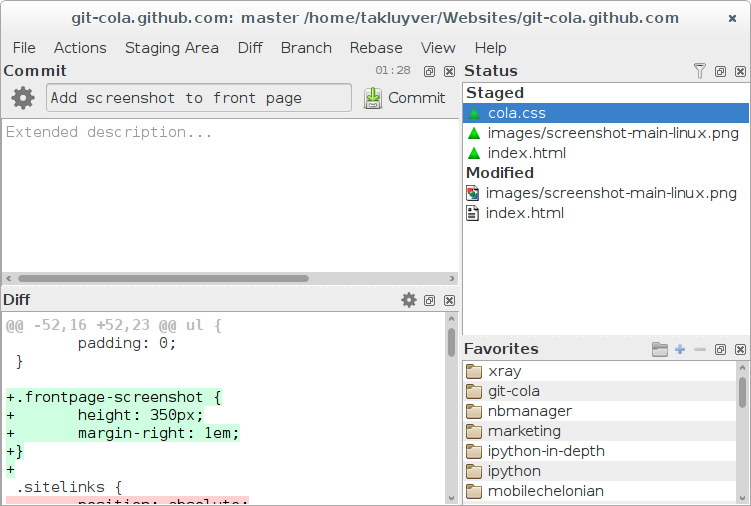
\includegraphics[width=0.9\linewidth]{images/git-cola.png}
\end{figure}
\end{frame}
